\section{eo\-Trunc\-Select$<$ EOT $>$ Class Template Reference}
\label{classeo_trunc_select}\index{eoTruncSelect@{eoTruncSelect}}
eo\-Trunc\-Select selects individuals after truncating the population using {\bf eo\-Select\-One}{\rm (p.\,\pageref{classeo_select_one})} as it's mechanism.  


{\tt \#include $<$eo\-Trunc\-Select.h$>$}

Inheritance diagram for eo\-Trunc\-Select$<$ EOT $>$::\begin{figure}[H]
\begin{center}
\leavevmode
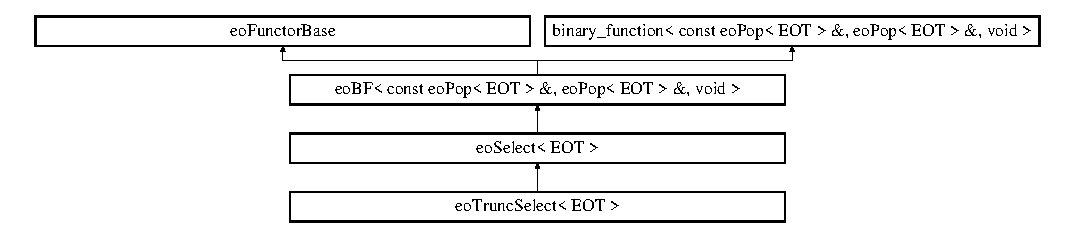
\includegraphics[height=2.75184cm]{classeo_trunc_select}
\end{center}
\end{figure}
\subsection*{Public Member Functions}
\begin{CompactItemize}
\item 
{\bf eo\-Trunc\-Select} ({\bf eo\-Select\-One}$<$ {\bf EOT} $>$ \&\_\-select, {\bf eo\-How\-Many} \_\-how\-Many)\label{classeo_trunc_select_a0}

\begin{CompactList}\small\item\em Ctor: from an {\bf eo\-Select}{\rm (p.\,\pageref{classeo_select})} (and an eo\-Many to tell how many are kept for selectino. \item\end{CompactList}\item 
virtual void {\bf operator()} (const {\bf eo\-Pop}$<$ {\bf EOT} $>$ \&\_\-source, {\bf eo\-Pop}$<$ {\bf EOT} $>$ \&\_\-dest)
\begin{CompactList}\small\item\em The implementation repeatidly selects an individual. \item\end{CompactList}\end{CompactItemize}
\subsection*{Private Attributes}
\begin{CompactItemize}
\item 
{\bf eo\-Select\-One}$<$ {\bf EOT} $>$ \& {\bf select}\label{classeo_trunc_select_r0}

\item 
{\bf eo\-How\-Many} {\bf how\-Many}\label{classeo_trunc_select_r1}

\end{CompactItemize}


\subsection{Detailed Description}
\subsubsection*{template$<$class EOT$>$ class eo\-Trunc\-Select$<$ EOT $>$}

eo\-Trunc\-Select selects individuals after truncating the population using {\bf eo\-Select\-One}{\rm (p.\,\pageref{classeo_select_one})} as it's mechanism. 

Therefore {\bf eo\-Select\-Many}{\rm (p.\,\pageref{classeo_select_many})} needs an {\bf eo\-Select\-One}{\rm (p.\,\pageref{classeo_select_one})} in its ctor It will use an eo\-How\-Mnay to determine the number of guys to keep, 



Definition at line 43 of file eo\-Trunc\-Select.h.

\subsection{Member Function Documentation}
\index{eoTruncSelect@{eo\-Trunc\-Select}!operator()@{operator()}}
\index{operator()@{operator()}!eoTruncSelect@{eo\-Trunc\-Select}}
\subsubsection{\setlength{\rightskip}{0pt plus 5cm}template$<$class EOT$>$ virtual void {\bf eo\-Trunc\-Select}$<$ {\bf EOT} $>$::operator() (const {\bf eo\-Pop}$<$ {\bf EOT} $>$ \& {\em \_\-source}, {\bf eo\-Pop}$<$ {\bf EOT} $>$ \& {\em \_\-dest})\hspace{0.3cm}{\tt  [inline, virtual]}}\label{classeo_trunc_select_a1}


The implementation repeatidly selects an individual. 

\begin{Desc}
\item[Parameters:]
\begin{description}
\item[{\em \_\-source}]the source population \item[{\em \_\-dest}]the resulting population (size of this population is the number of times {\bf eo\-Select\-One}{\rm (p.\,\pageref{classeo_select_one})} is called. It empties the destination and adds the selection into it) \end{description}
\end{Desc}


Implements {\bf eo\-BF$<$ const eo\-Pop$<$ EOT $>$ \&, eo\-Pop$<$ EOT $>$ \&, void $>$} {\rm (p.\,\pageref{classeo_b_f_a1})}.

Definition at line 56 of file eo\-Trunc\-Select.h.

References eo\-Select\-One$<$ EOT, Worth\-T $>$::setup().

The documentation for this class was generated from the following file:\begin{CompactItemize}
\item 
eo\-Trunc\-Select.h\end{CompactItemize}
